\section{Background and Motivation}
\label{sec:background}

\subsection{Existing resource management in Serverless}
\label{sec:background:resource-management}

% 1. serverless的资源管理模式: 静态资源分配管理
% 把 resource allocation 分为两个步骤,一个是节点-level的资源分配,即运行时的核数和内存,另一个cluster-level的资源分配,即是函数容器副本扩缩容和放置,即决定副本数量、并将容器放置到具体的节点。

Serverless computing has emerged as a popular cloud application paradigm. It allows
developers to focus on application logic by offloading infrastructure tasks. These
tasks include provisioning, scaling, and maintenance. This model is event-driven.
Users provide their code (functions) with basic resource specifications, like memory
and CPU limits. They also set simple triggers. The platform then provisions
sandboxed execution environments and manages their lifecycle. It also performs
on-demand autoscaling and offers pay-per-use billing. Effective resource management
in serverless platforms is essential to ensure performance, increase utilization, and minimize cost.

In practice, resource management in serverless platforms involves two main dimensions:
(1) per-instance resource configuration, which specifies the resource limits for each function
sandbox, and (2) per-function resource configuration, which encompasses autoscaling
(determining the number of instances to run) and instance placement (deciding where to position them in the cluster).
Currently, both configurations rely on static and uniform resource settings for each function,
which we detail as follows.

\parabf{Static runtime resource allocation.}
% 1) 静态的运行时资源配置:介绍 lambda 支持指定固定资源规格,及其对延迟和开销的影响,所以选取一个所有请求都不违背qos的配置
Existing serverless platforms~\cite{Doc:Azure_Functions_Hosting,
Doc:GCP_CloudRun_Mem, aws_lambda} and serverless research~\cite{ASPLOS21:FaasCache, shahrad2020serverless, wang2018peeking, pu2019shuffling}
allocate a uniform amount of resources for all instances of a given function. In AWS Lambda, a
developer specifies a memory size (e.g., 128 MB–10,240 MB), from which the
platform derives proportional vCPU and network bandwidth shares. Developers may
also set ephemeral storage per instance (default 512 MB, configurable up to
several GB). These limits remain fixed throughout the sandbox's lifetime.
Similar static per-instance specifications are used by Azure Functions and
Google Cloud Run~\cite{Doc:Azure_Functions_Hosting, Doc:GCP_CloudRun_Mem}. This
approach presumes uniform resource demand across function invocations.
Operators typically select the smallest configuration that satisfies the
function's QoS (e.g., latency SLO) to minimize costs.

%  已有工作: 运行时资源配置:根据 profile 进行 static 资源分配,在延迟和开销间做合理tradeoff,引用一些相关工作,如 
Optimizations on the static per-instance resource allocation focus on
profile-guided static tuning~\cite{aws_lambda_power_tuning,ASPLOS21:FaasCache, shahrad2020serverless, wang2018peeking, pu2019shuffling}
is common in FaaS: functions are profiled
across discrete memory tiers to obtain latency–cost curves, and the
cheapest configuration satisfying SLOs is selected. Provider tooling
automates this search, while studies characterize sensitivity and
per-function heterogeneity; research further leverages these profiles
to set memory/CPU reservations that minimize cost under QoS
constraints.

\parabf{Serverless sandbox autoscaling and placement based on static resource configuration.}
% 2)根据静态资源配置进行容器扩缩容放置:现有的 serverless 系统大多基于静态资源配置进行容器放置调度
% 仅容器启动、离开时比较资源:只需维护节点已分配资源和未分配资源总计,任务到来时可以分配到未分配资源>静态请求资源的节点上,更新已分配资源、未分配资源,函数容器销毁时释放资源、更新已分配资源、未分配资源即可
Existing serverless systems scale~\cite{aws_scaling_window, aws_scaling_eq,
knative_scaling} and place instances using each function’s
static per‑instance configuration. With uniform resources per sandbox, autoscalers
adjust replica counts from load signals, while the scheduler relies on simple
resource accounting: each node tracks allocated and available capacity.
A container is admitted to a node only if available is larger or equal to the
function’s static request (e.g., memory, vCPU); on placement the counters are updated,
and reverted on termination or eviction. These updates occur only at lifecycle events (start/stop).

% 已有工作:

% 第一段,函数容器副本数量:基于历史预测,引用文章
For autoscaling, recent systems research uses prediction to
right-size replicas and proactively prewarm functions. Shahrad et al.
analyze production traces and propose a per-function histogram policy
that jointly sets keep-alive and pre-warming windows, cutting cold
starts at lower cost \cite{shahrad2020serverless}. For workflows,
Orion models end-to-end SLOs in DAGs and prewarms downstream stages
with the right look-ahead \cite{ORION_MahgoubYSECB22}.

% 第二段(或二、三段),函数容器副本放置缓存亲和性、多资源综合考虑调度:考虑(先几句话说缓存为啥重要)缓存是否存在、多资源性质(即预备资源分配),引用文章
% 可以考虑,包含 FaasCache这种单机容器缓存管理, serverless workflow 相邻stage亲和放置,jiagu这种多节点协同缓存管理,引用更多文章
Recent advancements in placement strategies consider three main aspects: cache awareness,
heterogeneous resource, and data-affinity, improving cost-efficiency and latency in serverless systems.
Incorporating cache awareness helps to decrease costs and latency associated with cold starts.
Different instances can share certain memory states~\cite{SOCK_OakesYZHHAA18, li2022help},
allowing for rapid and cost-effective instance creation.
Moreover, considering heterogeneous resource awareness~\cite{RoyPT22, DuLJXZC22} in placement is critical,
as functions and resources exhibit heterogeneous characteristics.
This approach minimizes resource wastage and optimizes utilization.
Additionally, data-affinity aware placement strategies~\cite{Wukong_CarverZWAWC20, ORION_MahgoubYSECB22}
have been proposed for serverless workflows to reduce data transfer overheads between stages.


% 2. serverless 函数资源需求分析
\subsection{Function Resource Demand Analysis}
\label{sec:background:demand-analysis}

% 1) 函数资源占用的特点
\paraf{Resource Usage Variation Across Invocations.}
Invocations of the same serverless function can show significant differences in
resource consumption. For instance, analyzing CPU usage at the invocation level
for a representative function produces a wide empirical distribution, as shown in
Figure~\ref{fig:usage_variation}(a). This suggests that inputs, execution paths, and
runtime conditions greatly affect demand. To quantify this within-function variability,
we calculate the standard deviation of invocation-level resource usage for each function
as a measure of variability. Analyzing many functions, Figure~\ref{fig:usage_variation}(b)
displays the distribution of these per-function standard deviations; the notable presence
of high values indicates that substantial invocation-to-invocation variability is typical.
Similar patterns are observed for memory usage.

\begin{figure}[t]
  \centering
  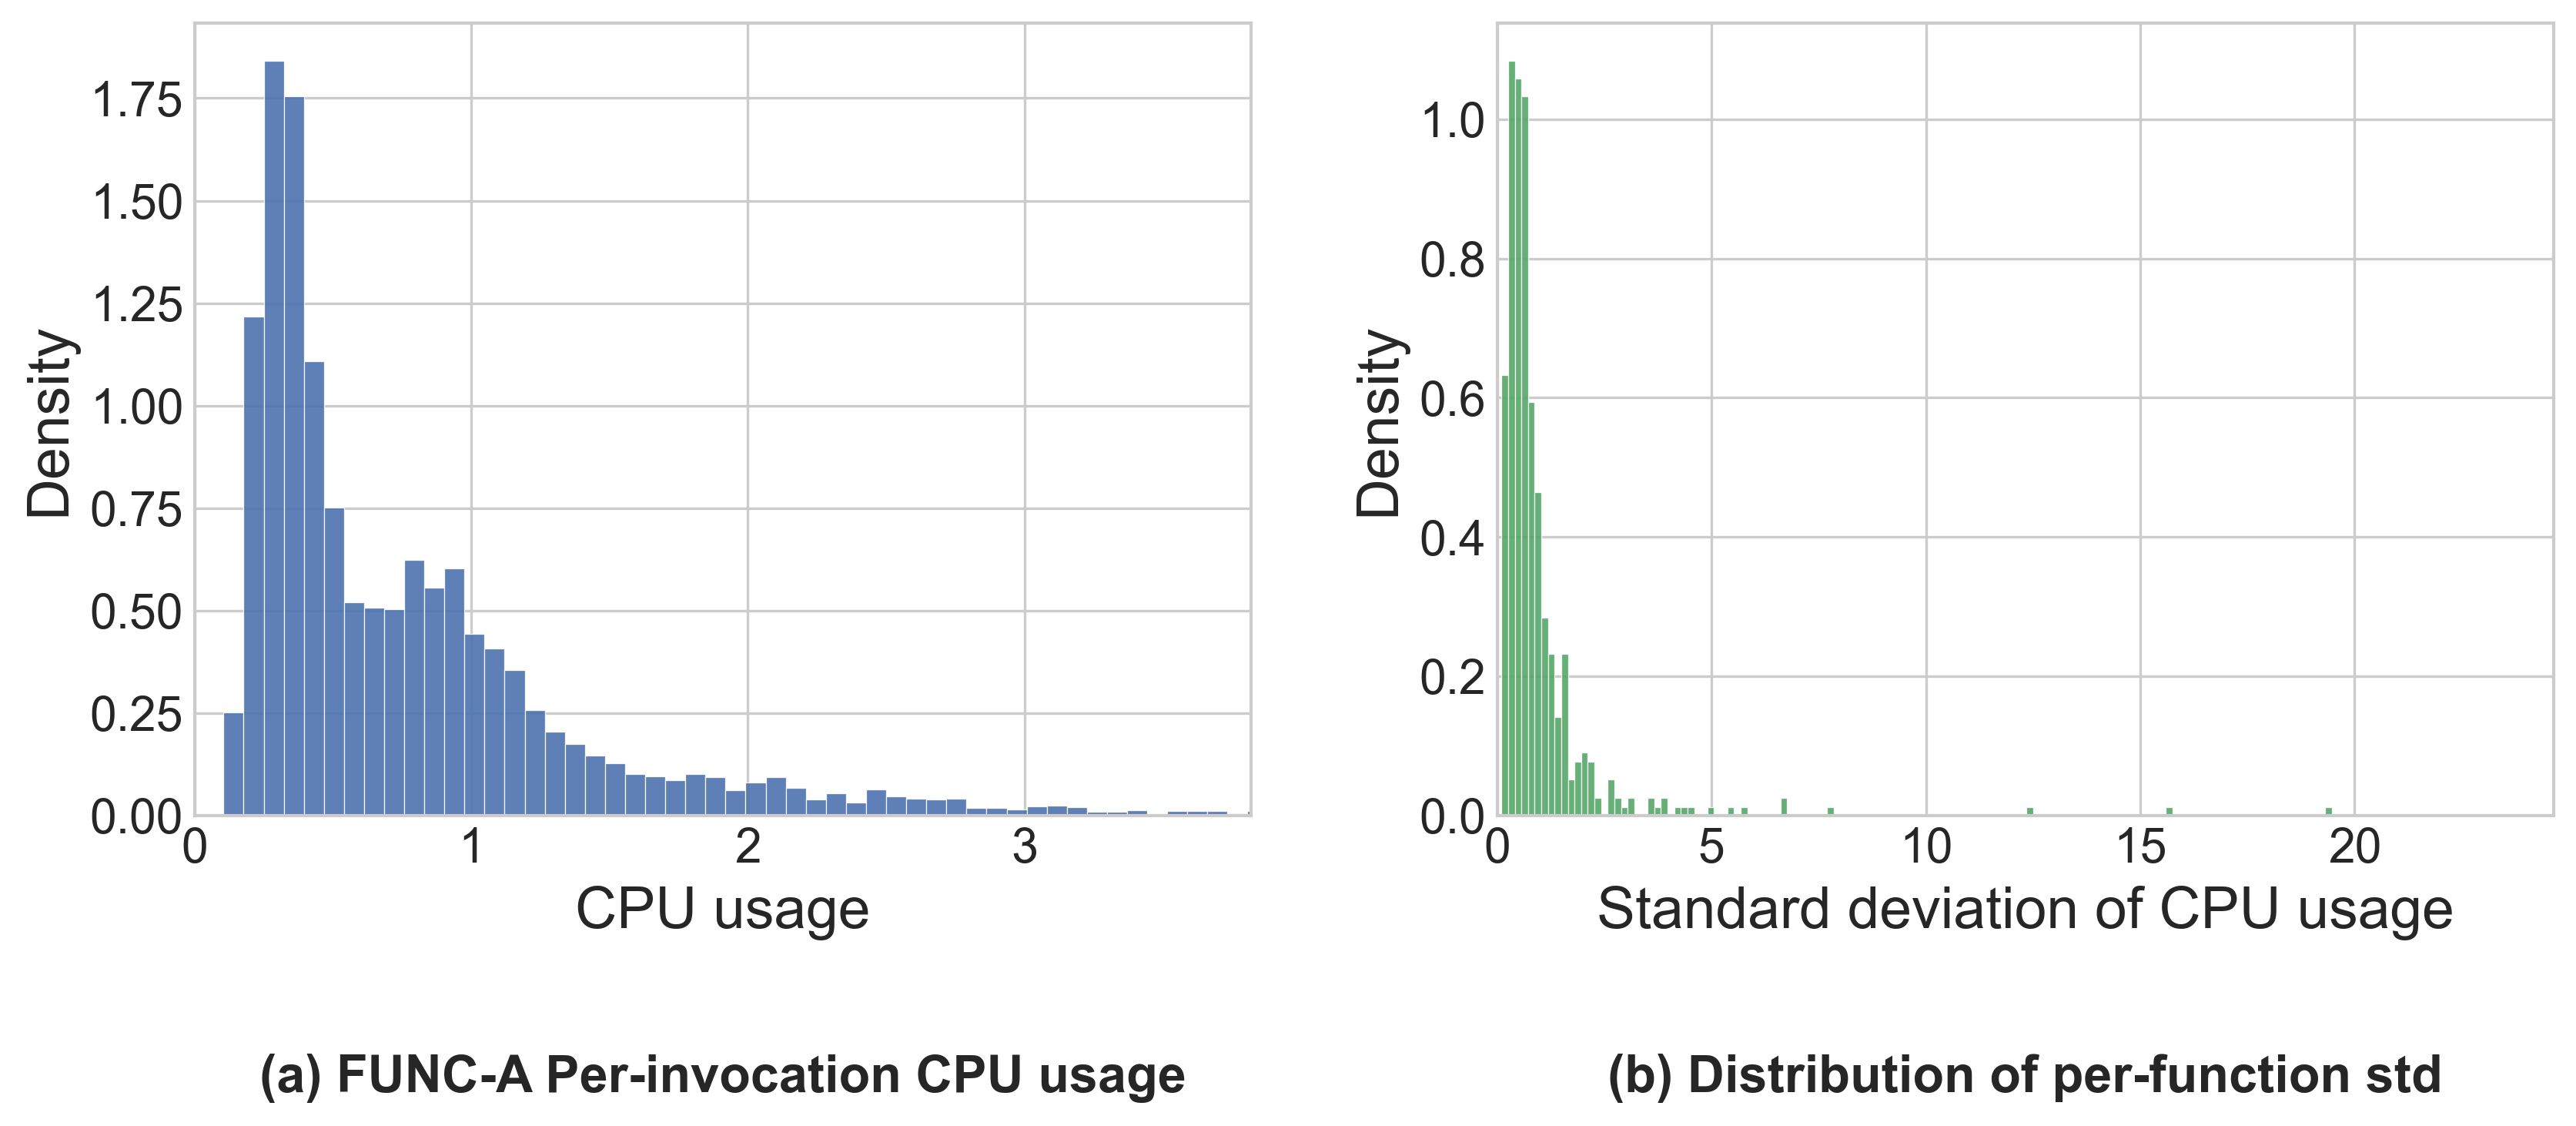
\includegraphics[width=1.0\linewidth]{figures/background/usage_variation.png}
  \caption{Resource usage variations of serverless function.}
  \label{fig:usage_variation}
\end{figure}

% 2) 现有调度方案的问题
\parabf{Drawback of existing solutions: Static resource allocation waste resources.}
Static, uniform per‑instance sizing ignores intra‑function resource usage variability.
When set to a high tier, most invocations are overprovisioned, wasting CPU/memory
and inflating cost. When set to a low tier, peak‑demand invocations are
underprovisioned, causing throttling, queuing, memory overflow.
Fixed sizing also worsens data locality and resource fragmentation.

% 3) Opportunity: 函数动态运行时资源调整 
% 现有容器框架支持动态运行时资源分配(具体机制或者接口),以及其好处(节省资源减少浪费)
\parabf{Opportunity: Dynamic in‑place runtime resource adjustment}
Dynamically aligning each invocation's resource needs with its sandbox allocation
absorbs bursts and handles intra-function heterogeneity, improving utilization and
reducing overprovisioning and SLO risks. Kubernetes supports in‑place vertical scaling
via Pod resize subresource, updating container {requests,limits} without recreation,
including both memory and CPU allocation adjustments. Memory scaling is achieved by modifying cgroup limits,
which dynamically changes the memory allocation for a running container without stopping it.
Similarly, CPU resources can be adjusted by altering cgroup CPU shares and quotas, allowing the kubelet
to allocate CPU cycles according to usage metrics and policy constraints \cite{Doc:K8s_Pod_Resize, Doc:K8s_CRI_Update}.
This ensures that all resources can be increased or decreased to respond to real-time demands.
A serverless control plane can utilize these features to dynamically adjust sandboxes for
both CPU and memory, optimizing resources while preserving state and improving cost and latency efficiency.

% 3. 动态资源分配的挑战

\subsection{Challenges in Dynamic Resource Allocation for Serverless Functions}
\label{sec:background:challenges}

% 1) 挑战1:资源分配+副本扩缩挑战:如何确定一个函数的容器的资源组合(比如1核1个、2核1个、3核1个),以便在高效利用资源的同时,满足函数的动态资源需求
% appeal for workload-split based 资源组合分配

\paraf{Challenge 1: Function Resource Configuration Portfolio.}
When configuring dynamic and non-uniform resource configurations for serverless
containers, it is essential to fit known workload patterns with an appropriate
portfolio of instance sizes. Improper sizing can lead to inefficiencies such as
resource overprovisioning, inflated costs, and potential violations of service
level objectives (SLOs). This appeals for a workload-splitting formulation that
divides the function's resource-usage distribution into distinct regions, as
illustrated by the histogram in Figure~\ref{fig:challenge1}. Each region can be
allocated a suitable instance size, forming a well-balanced resource
configuration portfolio based on its demand profile.

\begin{figure}[t]
  \centering
  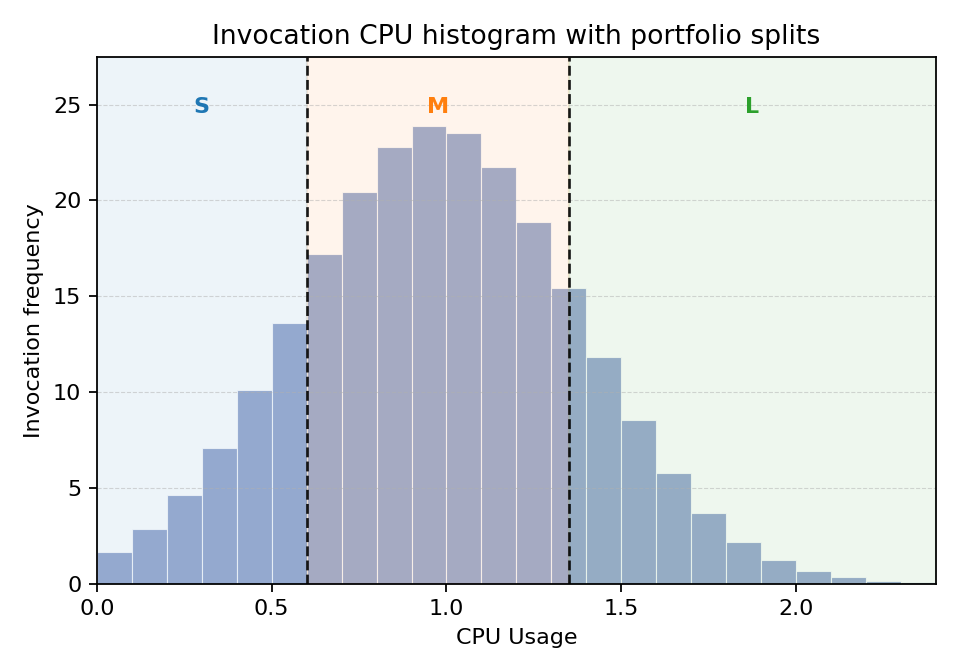
\includegraphics[width=0.9\linewidth]{figures/background/challenge1_mix.png}
  \caption{Workload-split based resource configuration portfolio for a function.}
  \label{fig:challenge1}
\end{figure}

% 2)挑战2:副本放置挑战:动态资源分配打破了原有的静态资源分配假设,容器的资源需求不再是固定的,不能仅在容器启动和销毁时考虑节点资源分配
% strawman solution:发生扩容剩余节点资源不足时直接evict其他同节点容器,但带来缓存损失,且可能放大(相对较大规格的容器扩容,可能一下需要evict多个小规格容器)
% appeal for Minimal-Disruption Placement Scaling with multi-resource balance awareness

\paraf{Challenge 2: Placement under Dynamic In-Place Resizing.} Dynamic in-place
resizing disrupts the fixed-size bin-packing model: a sandbox’s footprint may
expand while active, making node feasibility assessments at start/stop times
inadequate. A simplistic approach is to evict co-located sandboxes to make space
when upscaling faces insufficient capacity. However, this naive strategy risks
evicting other colocated function instances as resource demands rise. This is
especially problematic when a large upscale meets tight headroom, causing
eviction amplification: a single significant resize can trigger numerous evictions
of smaller colocated sandboxes, leading to cache losses and increased tail
latency. Additionally, fragmentation can occur when resource requests shrink.
These challenges can degrade utilization and throughput during dynamic swarming.

We require a minimal-disruption placement strategy that is aware of
multi-resource needs. It should favor in-place growth using precise headroom,
limit preemptions, and choose victims that maintain cache locality. Furthermore,
it should balance the CPU:memory mix per node to prevent fragmentation, employing
targeted micro-migrations only when they minimize overall disruption. Such policies
encourage managed churn, safeguard warm states, and enhance packing efficiency
and throughput during dynamic resizing.

% todo: 请按需加图

% \begin{figure}[t]
%   \centering
%   \begin{minipage}[t]{0.48\linewidth}
%     \centering
%     \includegraphics[width=\linewidth]
%     {figures/background/challenge2_eviction_amplification.png}
%     \vspace{2pt}
%     \small Left: Upsizing a large sandbox may evict many small ones
%     (amplification).
%   \end{minipage}\hfill
%   \begin{minipage}[t]{0.48\linewidth}
%     \centering
%     \includegraphics[width=\linewidth]
%     {figures/background/challenge2_stranding.png}
%     \vspace{2pt}
%     \small Right: Ignoring multi‑resource balance strands CPU or memory.
%   \end{minipage}
%   \caption{Challenge 2: Dynamic in‑place scaling complicates placement under
%   tight capacity.}
%   \label{fig:challenge2_placement}
% \end{figure}

\begin{figure}[t]
  \centering
  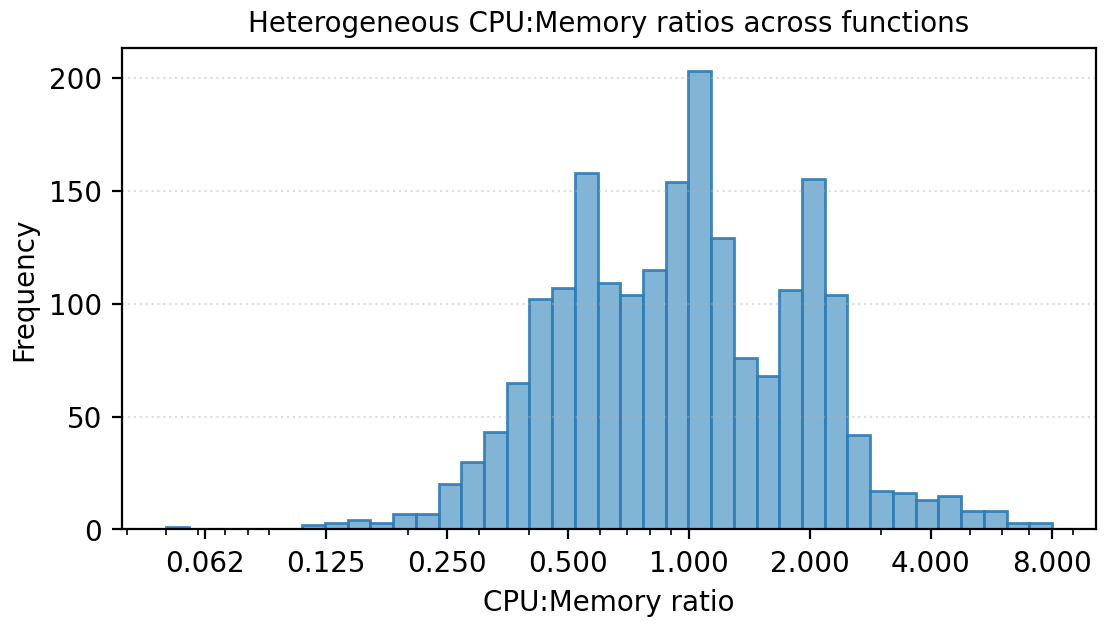
\includegraphics[width=0.7\linewidth]
  {figures/background/cpu_mem_ratio_hist.png}
  \caption{Heterogeneous CPU:memory ratios across functions.}
  \label{fig:cpu_mem_ratio_hist}
\end{figure}


% 3)挑战3:资源缩容本身有成本挑战:扩容成本低,但缩容成本高。对于请求量没那么大的函数有难度。
%Second, dynamic resource adjustment mechanisms introduce non-negligible overhead.
%Specifically, while increasing a container's resource capacity is a relatively fast operation, decreasing it is often much slower.
%For example, reducing the memory capacity of a container requires reclaiming memory pages, which incurs substantial latency.
%As resource adjustment occurs on the critical path of request execution, this latency directly increases the end-to-end request handling time.
% add overhead detail

% 对于请求量没那么大的函数
% strawman 1: 起很多副本,细致应对不同资源需求,但导致大量浪费
% strawman 2:只起少量副本,一会儿扩一会儿缩,但频繁调整带来高开销
% appeal for(opportunity): Vertical Scaling-Based Task Scheduling Algorithm,即按请求资源量从小到大reorder请求,使得单容器能从小到大单调递增扩容,然后只减少一次到很小,循环往复
\paraf{Challenge 3: Cost of Downsizing.} Dynamic in-place
scaling is asymmetric: upsizing is swift, but downsizing incurs costs. Increasing
the CPU quota takes immediate effect, whereas reducing memory triggers cgroup
reclamation, page-cache eviction, and compaction, potentially stalling both
runtime and kernel. Since resizing affects the request path, slow reclaim
increases tail latency and queueing. Concurrent shrinking actions can cause
reclaim storms, lowering node throughput even when average capacity suffices.

Two naive solutions struggle with bursty, diverse functions. First, over-provision
numerous replicas, each fixed to a narrow size band, to avoid resizing; this
squanders headroom and considerably harms utilization due to over-provisioning.
Second, operate few replicas and resize per request; this frequent adjustment
incurs reclaim costs repeatedly, disrupts page cache and JIT/heap state, and
increases scheduler interference. Both approaches decrease utilization and system
throughput, negating the advantages of dynamic scaling.

We propose a vertical-scaling-aware scheduler that orders invocations by predicted
demand within short batching windows. Each sandbox handles small, then medium,
then large requests, growing steadily and shrinking at most once per window during
quiescence. This approach amortizes reclamation, maintains warm state, and
alleviates pressure. Figure~\ref{fig:vertical_scaling_scheduling} demonstrates
the benefits of this method over naive resizing with FIFO scheduling. By reordering
requests, the scheduler reduces downsizing overheads by 33.3\%, leading to lower
overall latency and higher system throughput.
\begin{figure}[t]
  \centering
  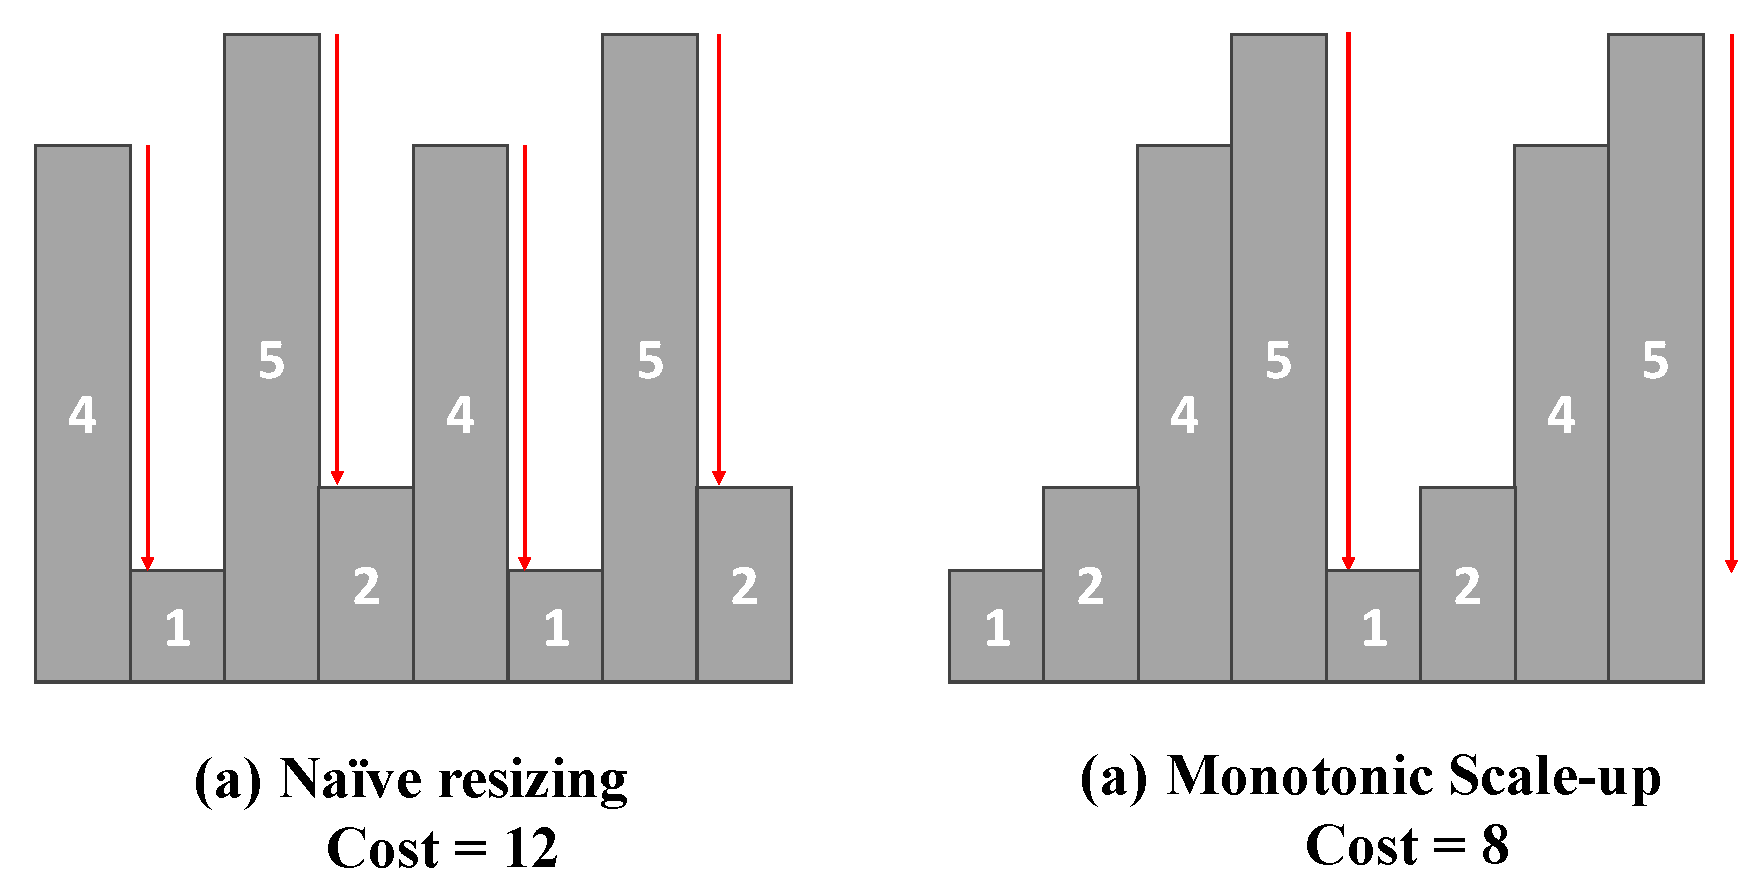
\includegraphics[width=1.0\linewidth]
  {figures/background/vertical.pdf}
  \caption{Vertical scaling-based task scheduling mitigates downsizing overhead
  by reordering requests.}
  \label{fig:vertical_scaling_scheduling}
\end{figure}

% # 本文优化目标(场景:高负载、高并发,核心目标:资源利用率和任务吞吐量)